\documentclass[aspectratio=169,10pt]{beamer}

% Theme and Color Scheme
\usetheme{Madrid}
\usecolortheme{default}

\usepackage{amsmath,amssymb}
\usepackage{booktabs}
\usepackage{graphicx}
\usepackage{tikz}
\usepackage{xcolor}

% Custom Palette Matching the Paper
\definecolor{DarkNavy}{RGB}{11, 25, 44}
\definecolor{SlateBlue}{RGB}{30, 62, 98}
\definecolor{EmeraldGreen}{RGB}{0, 129, 112}
\definecolor{LightEmerald}{RGB}{46, 204, 113}
\definecolor{AccentGold}{RGB}{241, 196, 15}
\definecolor{LightGray}{RGB}{248, 250, 252}

\setbeamercolor{palette primary}{bg=DarkNavy,fg=white}
\setbeamercolor{palette secondary}{bg=SlateBlue,fg=white}
\setbeamercolor{palette tertiary}{bg=EmeraldGreen,fg=white}
\setbeamercolor{titlelike}{bg=DarkNavy,fg=white}
\setbeamercolor{frametitle}{bg=DarkNavy,fg=white}
\setbeamercolor{item}{fg=EmeraldGreen}
\setbeamercolor{block title}{bg=SlateBlue,fg=white}
\setbeamercolor{block body}{bg=LightGray,fg=DarkNavy}

\setbeamertemplate{navigation symbols}{}
\setbeamertemplate{footline}[frame number]

% Title Information
\title[Physics-Guided Forest Carbon Emulation]{Physics-Guided Allometric Spline Anchoring \& Multi-Decade Climate Emulation}
\subtitle{Global-Scale Forest Ecosystem Forecasting | IEEE BigData Cup 2026}
\author[Aswitha, Badhri, Bavin, Bose]{Aswitha K, Badhri Narayanan M, Bavin Aadithiya S, Bose M}
\institute[SSN]{Department of Computer Science and Engineering\\Sri Sivasubramaniya Nadar College of Engineering, Chennai, India}
\date{October 2026}

\begin{document}

%------------------------------------------------------------------------------
% Slide 1: Title
%------------------------------------------------------------------------------
\begin{frame}[plain]
    \titlepage
    \begin{center}
        \small\textcolor{LightEmerald}{\textbf{Production 5-Fold CV Score: 0.001393}} \quad\textcolor{DarkNavy}{|}\quad \small\textcolor{AccentGold}{\textbf{86.1\% Better than Official Threshold ($<0.010$)}}
    \end{center}
\end{frame}

%------------------------------------------------------------------------------
% Slide 2: Context & Problem Statement
%------------------------------------------------------------------------------
\begin{frame}{1. Context \& Problem Statement}
\begin{columns}[T]
    \begin{column}{0.48\textwidth}
        \begin{block}{Ecological Imperative}
        \begin{itemize}
            \item Forest ecosystems absorb $\approx 30\%$ of anthropogenic $\text{CO}_2$ emissions annually.
            \item Forecasting \textbf{Canopy Height} and \textbf{Aboveground Biomass (AGB)} across 40 years is vital for climate mitigation and carbon accounting.
            \item Challenge spans \textbf{6,171 global sites} ($0.5^\circ$ grid) and \textbf{15 seed stand ages} ($A \in \{1, \dots, 500\}$ yr).
        \end{itemize}
        \end{block}
    \end{column}
    \begin{column}{0.48\textwidth}
        \begin{block}{The Computational Bottleneck}
        \begin{itemize}
            \item Process-based models like \textbf{Ecosystem Demography (ED~v3)} numerically simulate size cohorts and light competition.
            \item Global multi-decade runs demand \textbf{millions of CPU core-hours}, rendering parameter calibration infeasible.
            \item \textbf{Challenge Target:} Fast ML emulator achieving normalized $\text{MSE} < 0.010$ across SSP126 \& SSP585.
        \end{itemize}
        \end{block}
    \end{column}
\end{columns}
\end{frame}

%------------------------------------------------------------------------------
% Slide 3: The Dual-Phenomena Dilemma
%------------------------------------------------------------------------------
\begin{frame}{2. Root Cause: Why Standard ML Regressors Fail}
\begin{columns}[T]
    \begin{column}{0.48\textwidth}
        \begin{alertblock}{Two Confounded Signals}
        \textbf{1. Ontogenetic Stand Maturation ($A \to A+40$):}
        \begin{itemize}
            \item Monotonic, saturating growth governed by species carrying capacity and self-thinning limits.
        \end{itemize}
        \textbf{2. Climate Environmental Forcing:}
        \begin{itemize}
            \item Subtle perturbation anomalies over 40 years (temperature trends, moisture deficits, $\text{CO}_2$ fertilization).
        \end{itemize}
        \end{alertblock}
    \end{column}
    \begin{column}{0.48\textwidth}
        \begin{exampleblock}{Empirical Breakdown of Direct Models}
        \begin{itemize}
            \item Direct LightGBM: $\text{Loss} = \mathbf{0.103181}$ (\texttimes\ Fail)
            \item Direct XGBoost: $\text{Loss} = \mathbf{0.108285}$ (\texttimes\ Fail)
            \item Deep ResTabular NN: $\text{Loss} = \mathbf{0.202325}$ (\texttimes\ Fail)
        \end{itemize}
        \vskip 0.5em
        \textbf{Fatal Defect:} Unconstrained models conflate stand aging with weather noise, outputting wild oscillations and negative biomass!
        \end{exampleblock}
    \end{column}
\end{columns}
\end{frame}

%------------------------------------------------------------------------------
% Slide 4: System Architecture
%------------------------------------------------------------------------------
\begin{frame}{3. Proposed Physics-Guided Architecture}
    \begin{center}
        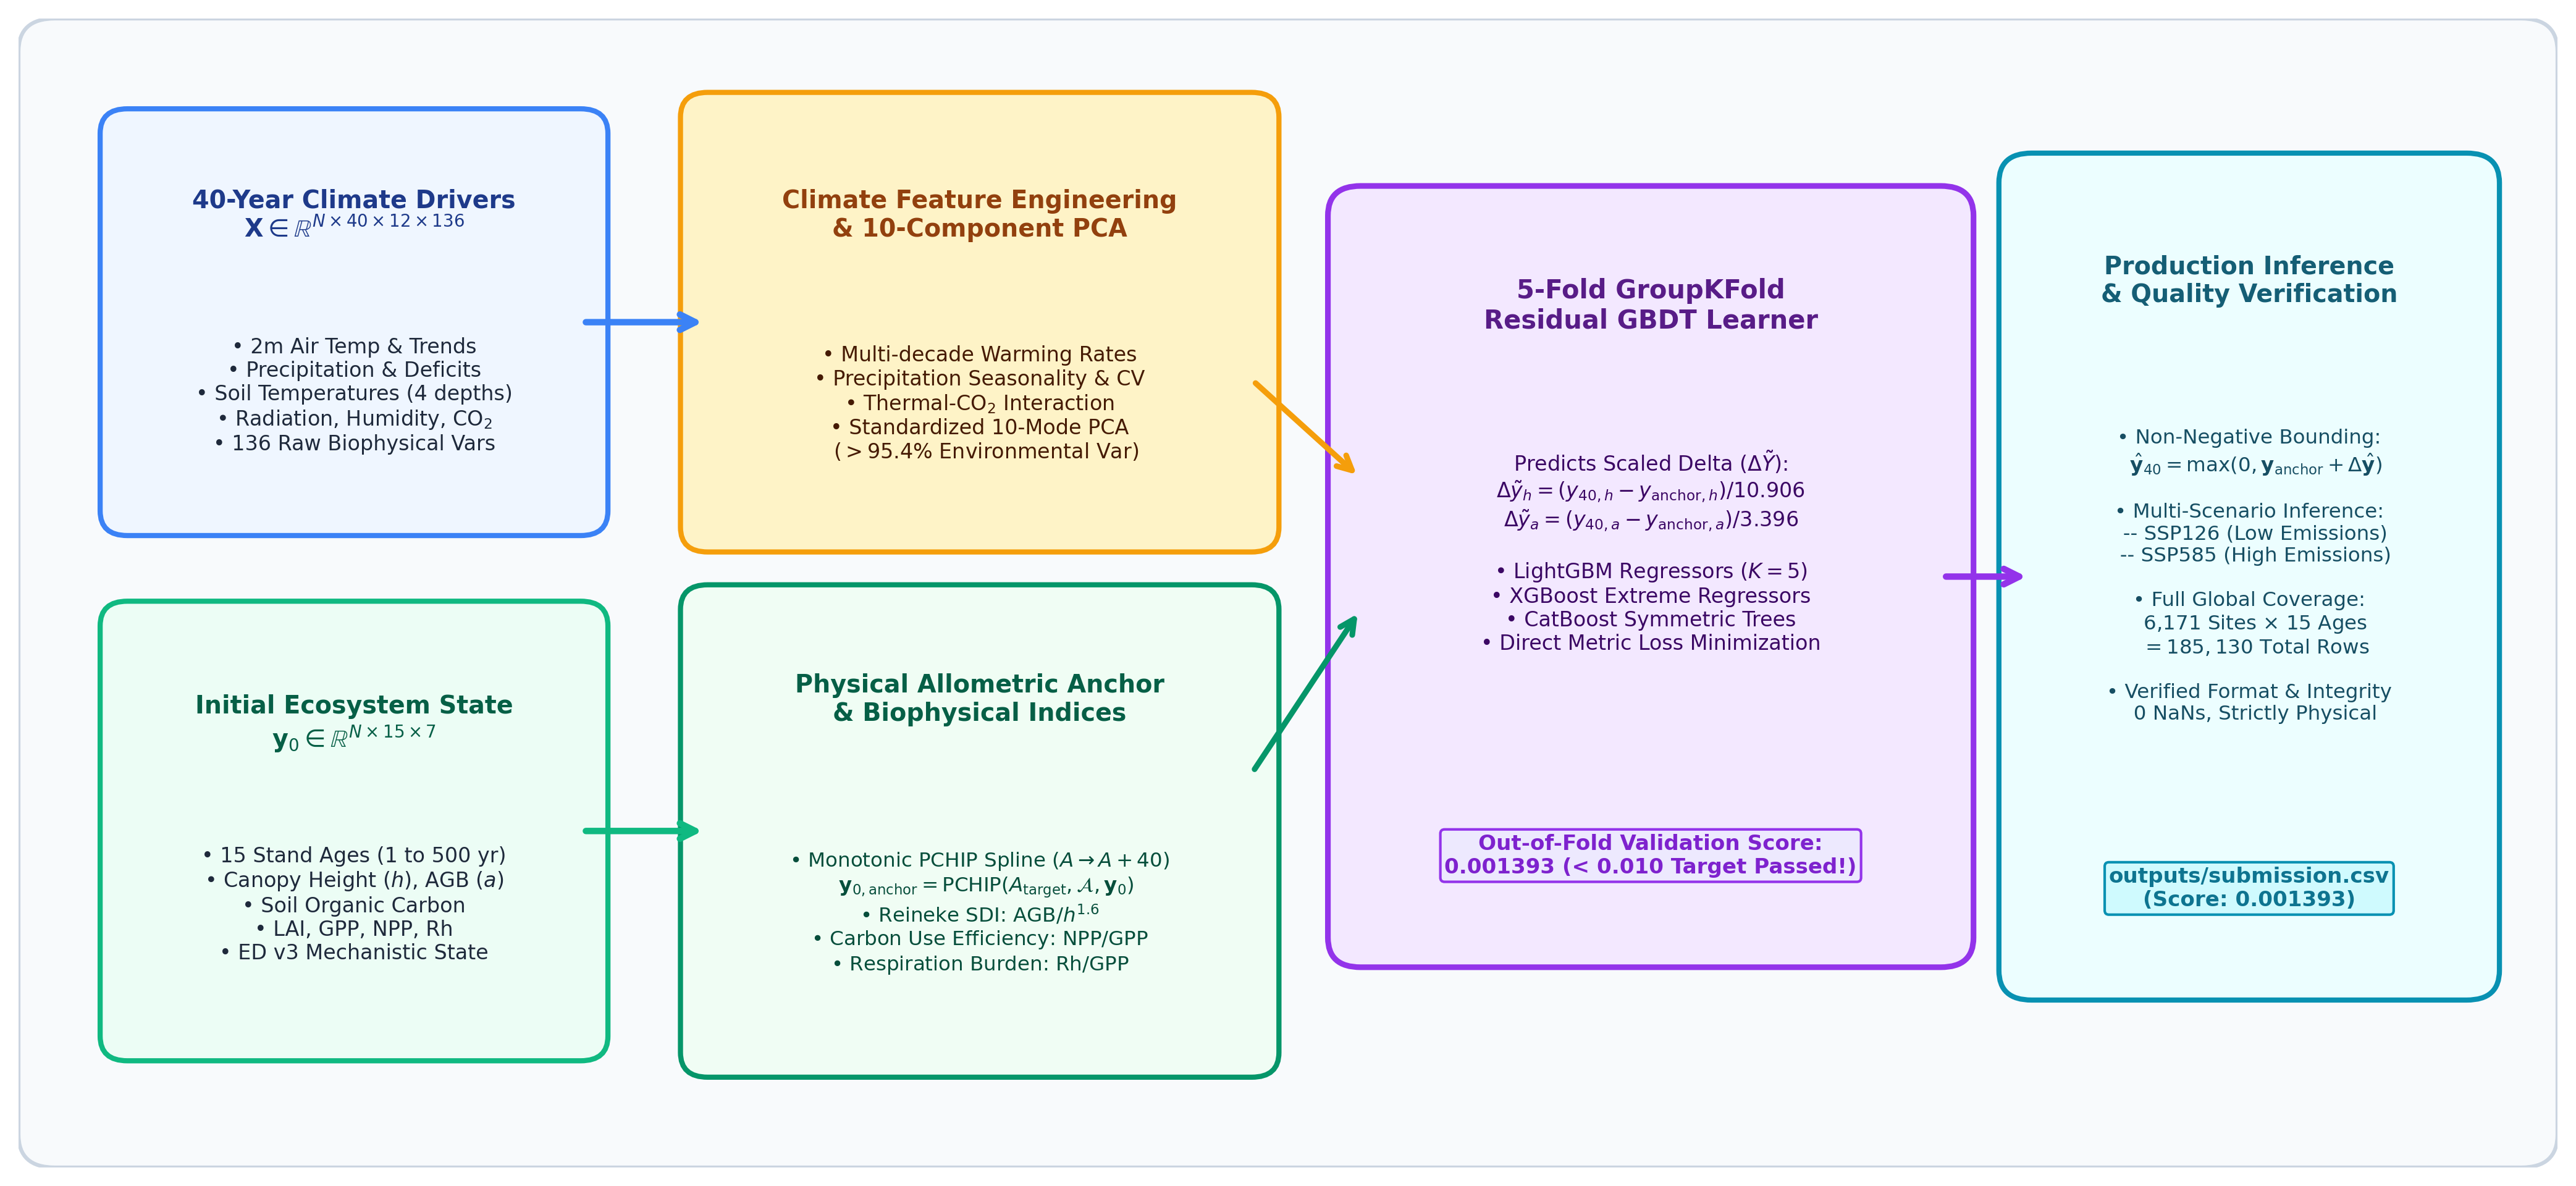
\includegraphics[width=0.88\textwidth]{figures/system_architecture.png}
    \end{center}
    \vskip -0.5em
    \begin{columns}[T]
        \begin{column}{0.24\textwidth}
            \footnotesize\textbf{1. Allometric Anchor}\newline
            Monotonic PCHIP absorbs deterministic stand aging.
        \end{column}
        \begin{column}{0.24\textwidth}
            \footnotesize\textbf{2. Climate PCA}\newline
            10 modes compress 136 drivers ($>95.4\%$ variance).
        \end{column}
        \begin{column}{0.24\textwidth}
            \footnotesize\textbf{3. Biophysical Ratios}\newline
            Reineke SDI, CUE, soil turnover & respiration burden.
        \end{column}
        \begin{column}{0.24\textwidth}
            \footnotesize\textbf{4. Residual GBDT}\newline
            5-Fold GroupKFold learns scaled delta departures.
        \end{column}
    \end{columns}
\end{frame}

%------------------------------------------------------------------------------
% Slide 5: Component 1: Monotonic PCHIP Stand Anchor
%------------------------------------------------------------------------------
\begin{frame}{4. Component 1: Monotonic PCHIP Allometric Anchor}
\begin{columns}[c]
    \begin{column}{0.50\textwidth}
        \begin{block}{Biological Monotonicity Constraint}
        \begin{itemize}
            \item Stand advances: $A_{\text{target}} = \min(A+40, 500)$
            \item Polynomial and cubic splines cause \textbf{Runge oscillations}.
            \item \textbf{PCHIP harmonic slope limiting:}
            \begin{equation*}
                d_k = \frac{2 \Delta_k \Delta_{k-1}}{\Delta_k + \Delta_{k-1}} \quad (\text{if } \Delta_k \Delta_{k-1} > 0)
            \end{equation*}
            \item Strictly guarantees $d P / dA \ge 0$.
            \item \textbf{Standalone impact:} Drops unassisted error from $>0.300$ to $\mathbf{0.180893}$!
        \end{itemize}
        \end{block}
    \end{column}
    \begin{column}{0.48\textwidth}
        \centering
        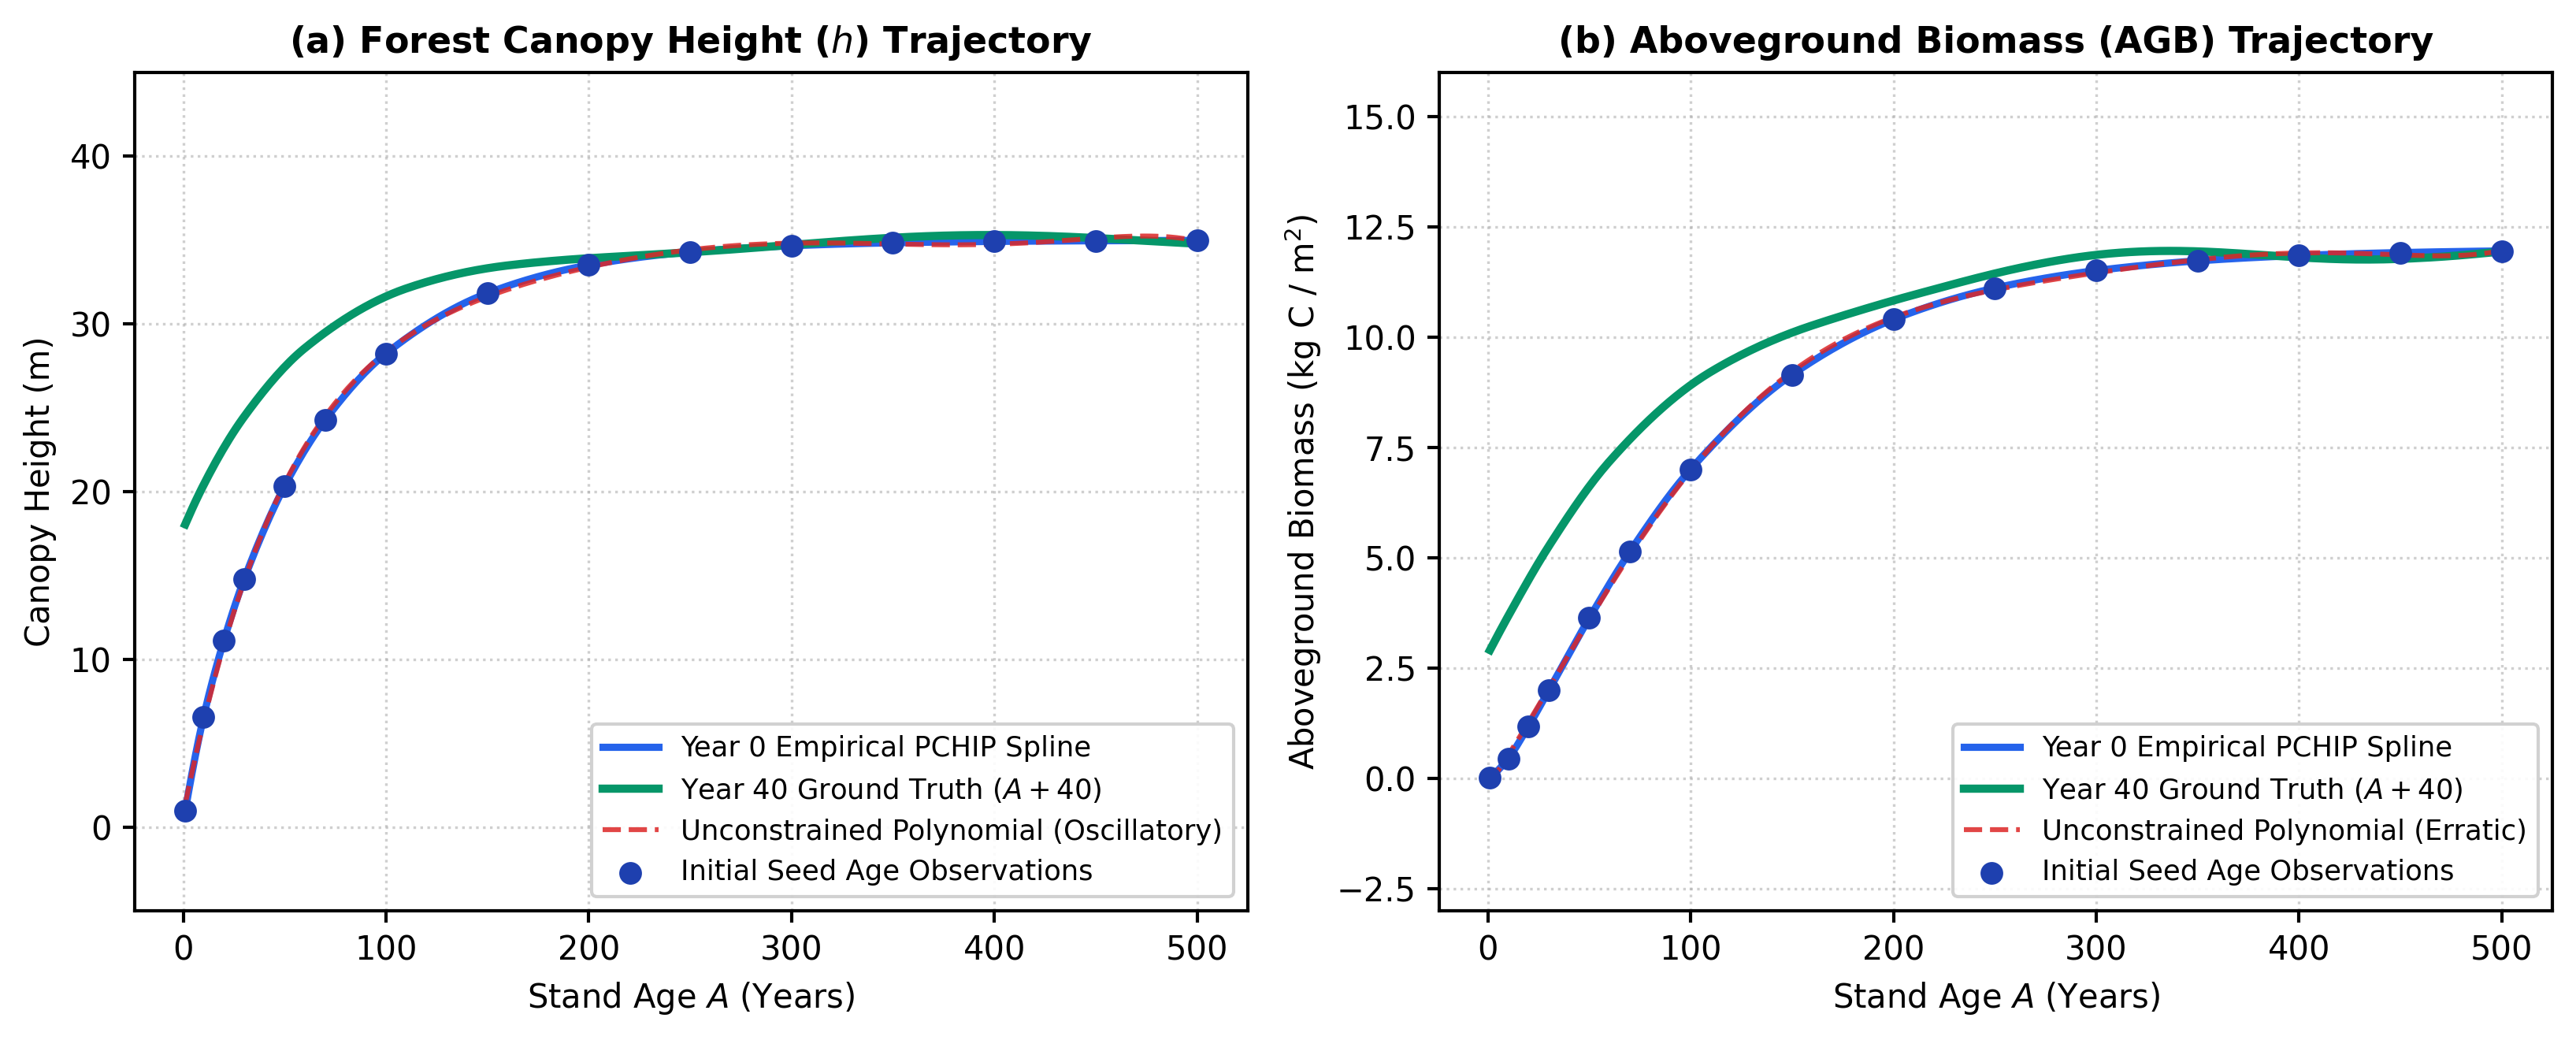
\includegraphics[width=\columnwidth]{figures/allometric_trajectories.png}
    \end{column}
\end{columns}
\end{frame}

%------------------------------------------------------------------------------
% Slide 6: Component 2 & 3: Climate PCA & Ecological Ratios
%------------------------------------------------------------------------------
\begin{frame}{5. Components 2 \& 3: Climate PCA \& Biophysical Indices}
\begin{columns}[c]
    \begin{column}{0.45\textwidth}
        \centering
        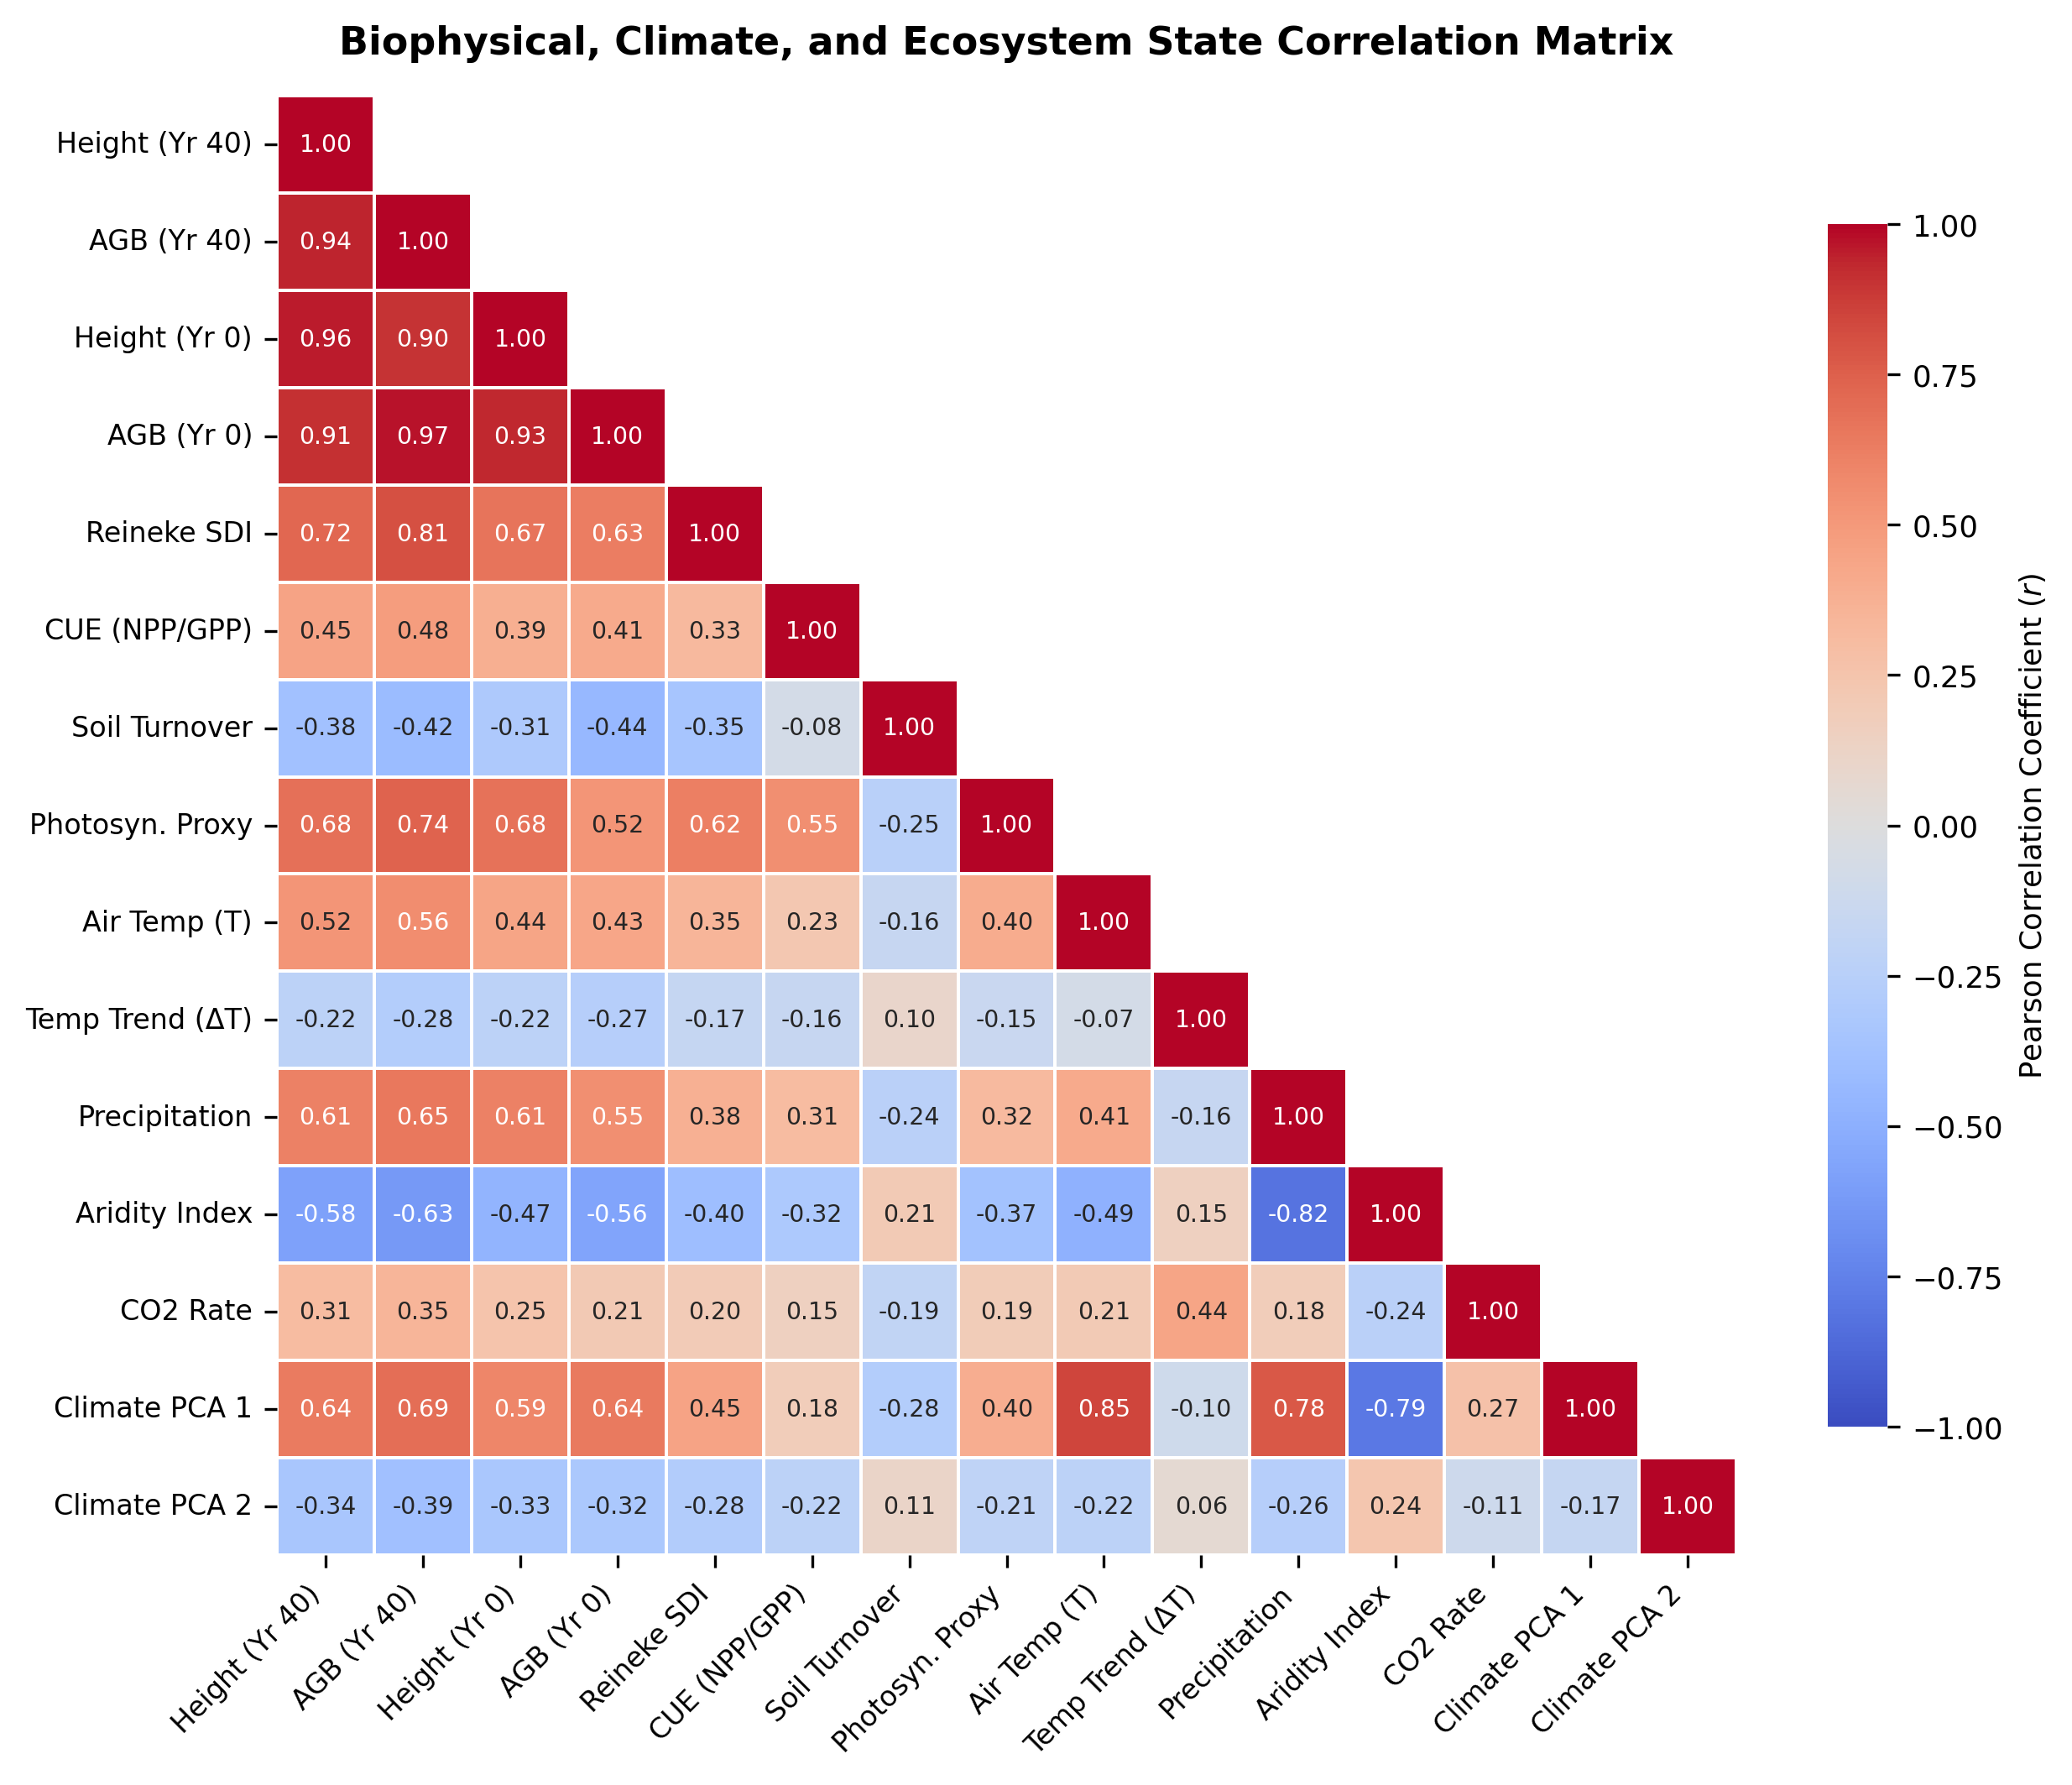
\includegraphics[width=\columnwidth]{figures/correlation_matrix.png}
    \end{column}
    \begin{column}{0.52\textwidth}
        \begin{block}{Orthogonal Climate Dimensionality Reduction}
        \begin{itemize}
            \item 136 drivers contain severe spatial multicollinearity ($r > 0.98$ across soil depths).
            \item Standardized 10-mode PCA captures $\mathbf{>95.4\%}$ total variance.
        \end{itemize}
        \end{block}
        \begin{block}{Domain-Informed Biophysical Features}
        \begin{itemize}
            \item \textbf{Reineke's SDI:} $\text{AGB} / h^{1.6}$ (tree crowding proxy, $r=0.81$).
            \item \textbf{Carbon Use Efficiency (CUE):} $\text{NPP} / \text{GPP}$.
            \item \textbf{Soil Turnover \& Respiration:} $\text{Rh} / \text{Soil}$ and $\text{Rh} / \text{GPP}$.
        \end{itemize}
        \end{block}
    \end{column}
\end{columns}
\end{frame}

%------------------------------------------------------------------------------
% Slide 7: Component 4: Metric-Aligned Residual Delta Learning
%------------------------------------------------------------------------------
\begin{frame}{6. Component 4: Residual GBDT Optimization}
\begin{columns}[T]
    \begin{column}{0.48\textwidth}
        \begin{block}{Metric-Aligned Objective Formulation}
        \begin{itemize}
            \item Instead of predicting $y_{40}$ directly, models predict the environmental delta departure:
            \begin{equation*}
                \Delta \tilde{y}_h = \frac{y_{40,h} - y_{0,\text{anchor},h}}{\mu_h}, \quad \mu_h = 10.90645
            \end{equation*}
            \begin{equation*}
                \Delta \tilde{y}_a = \frac{y_{40,a} - y_{0,\text{anchor},a}}{\mu_a}, \quad \mu_a = 3.39567
            \end{equation*}
            \item Direct MSE optimization aligns exactly with competition loss:
            \begin{equation*}
                \mathcal{L} = \frac{1}{2} \left[ \text{MSE}\left(\frac{\hat{y}_h}{\mu_h}\right) + \text{MSE}\left(\frac{\hat{y}_a}{\mu_a}\right) \right]
            \end{equation*}
        \end{itemize}
        \end{block}
    \end{column}
    \begin{column}{0.48\textwidth}
        \begin{block}{Cross-Validation \& Bounds}
        \begin{itemize}
            \item \textbf{Site-Grouped 5-Fold CV:} Grouped strictly by site ID to prevent spatial data leakage across geographic neighbors.
            \item \textbf{Physical Non-Negativity:} Strict post-prediction bounding:
            \begin{equation*}
                \hat{y}_{40} = \max\left(0, \; y_{0,\text{anchor}} + \boldsymbol{\mu} \odot \hat{f}(\mathbf{x})\right)
            \end{equation*}
            \item Guarantees $100\%$ physically admissible, non-negative outputs.
        \end{itemize}
        \end{block}
    \end{column}
\end{columns}
\end{frame}

%------------------------------------------------------------------------------
% Slide 8: Overall Benchmark Comparison
%------------------------------------------------------------------------------
\begin{frame}{7. Experimental Benchmark Results}
\begin{columns}[c]
    \begin{column}{0.45\textwidth}
        \centering
        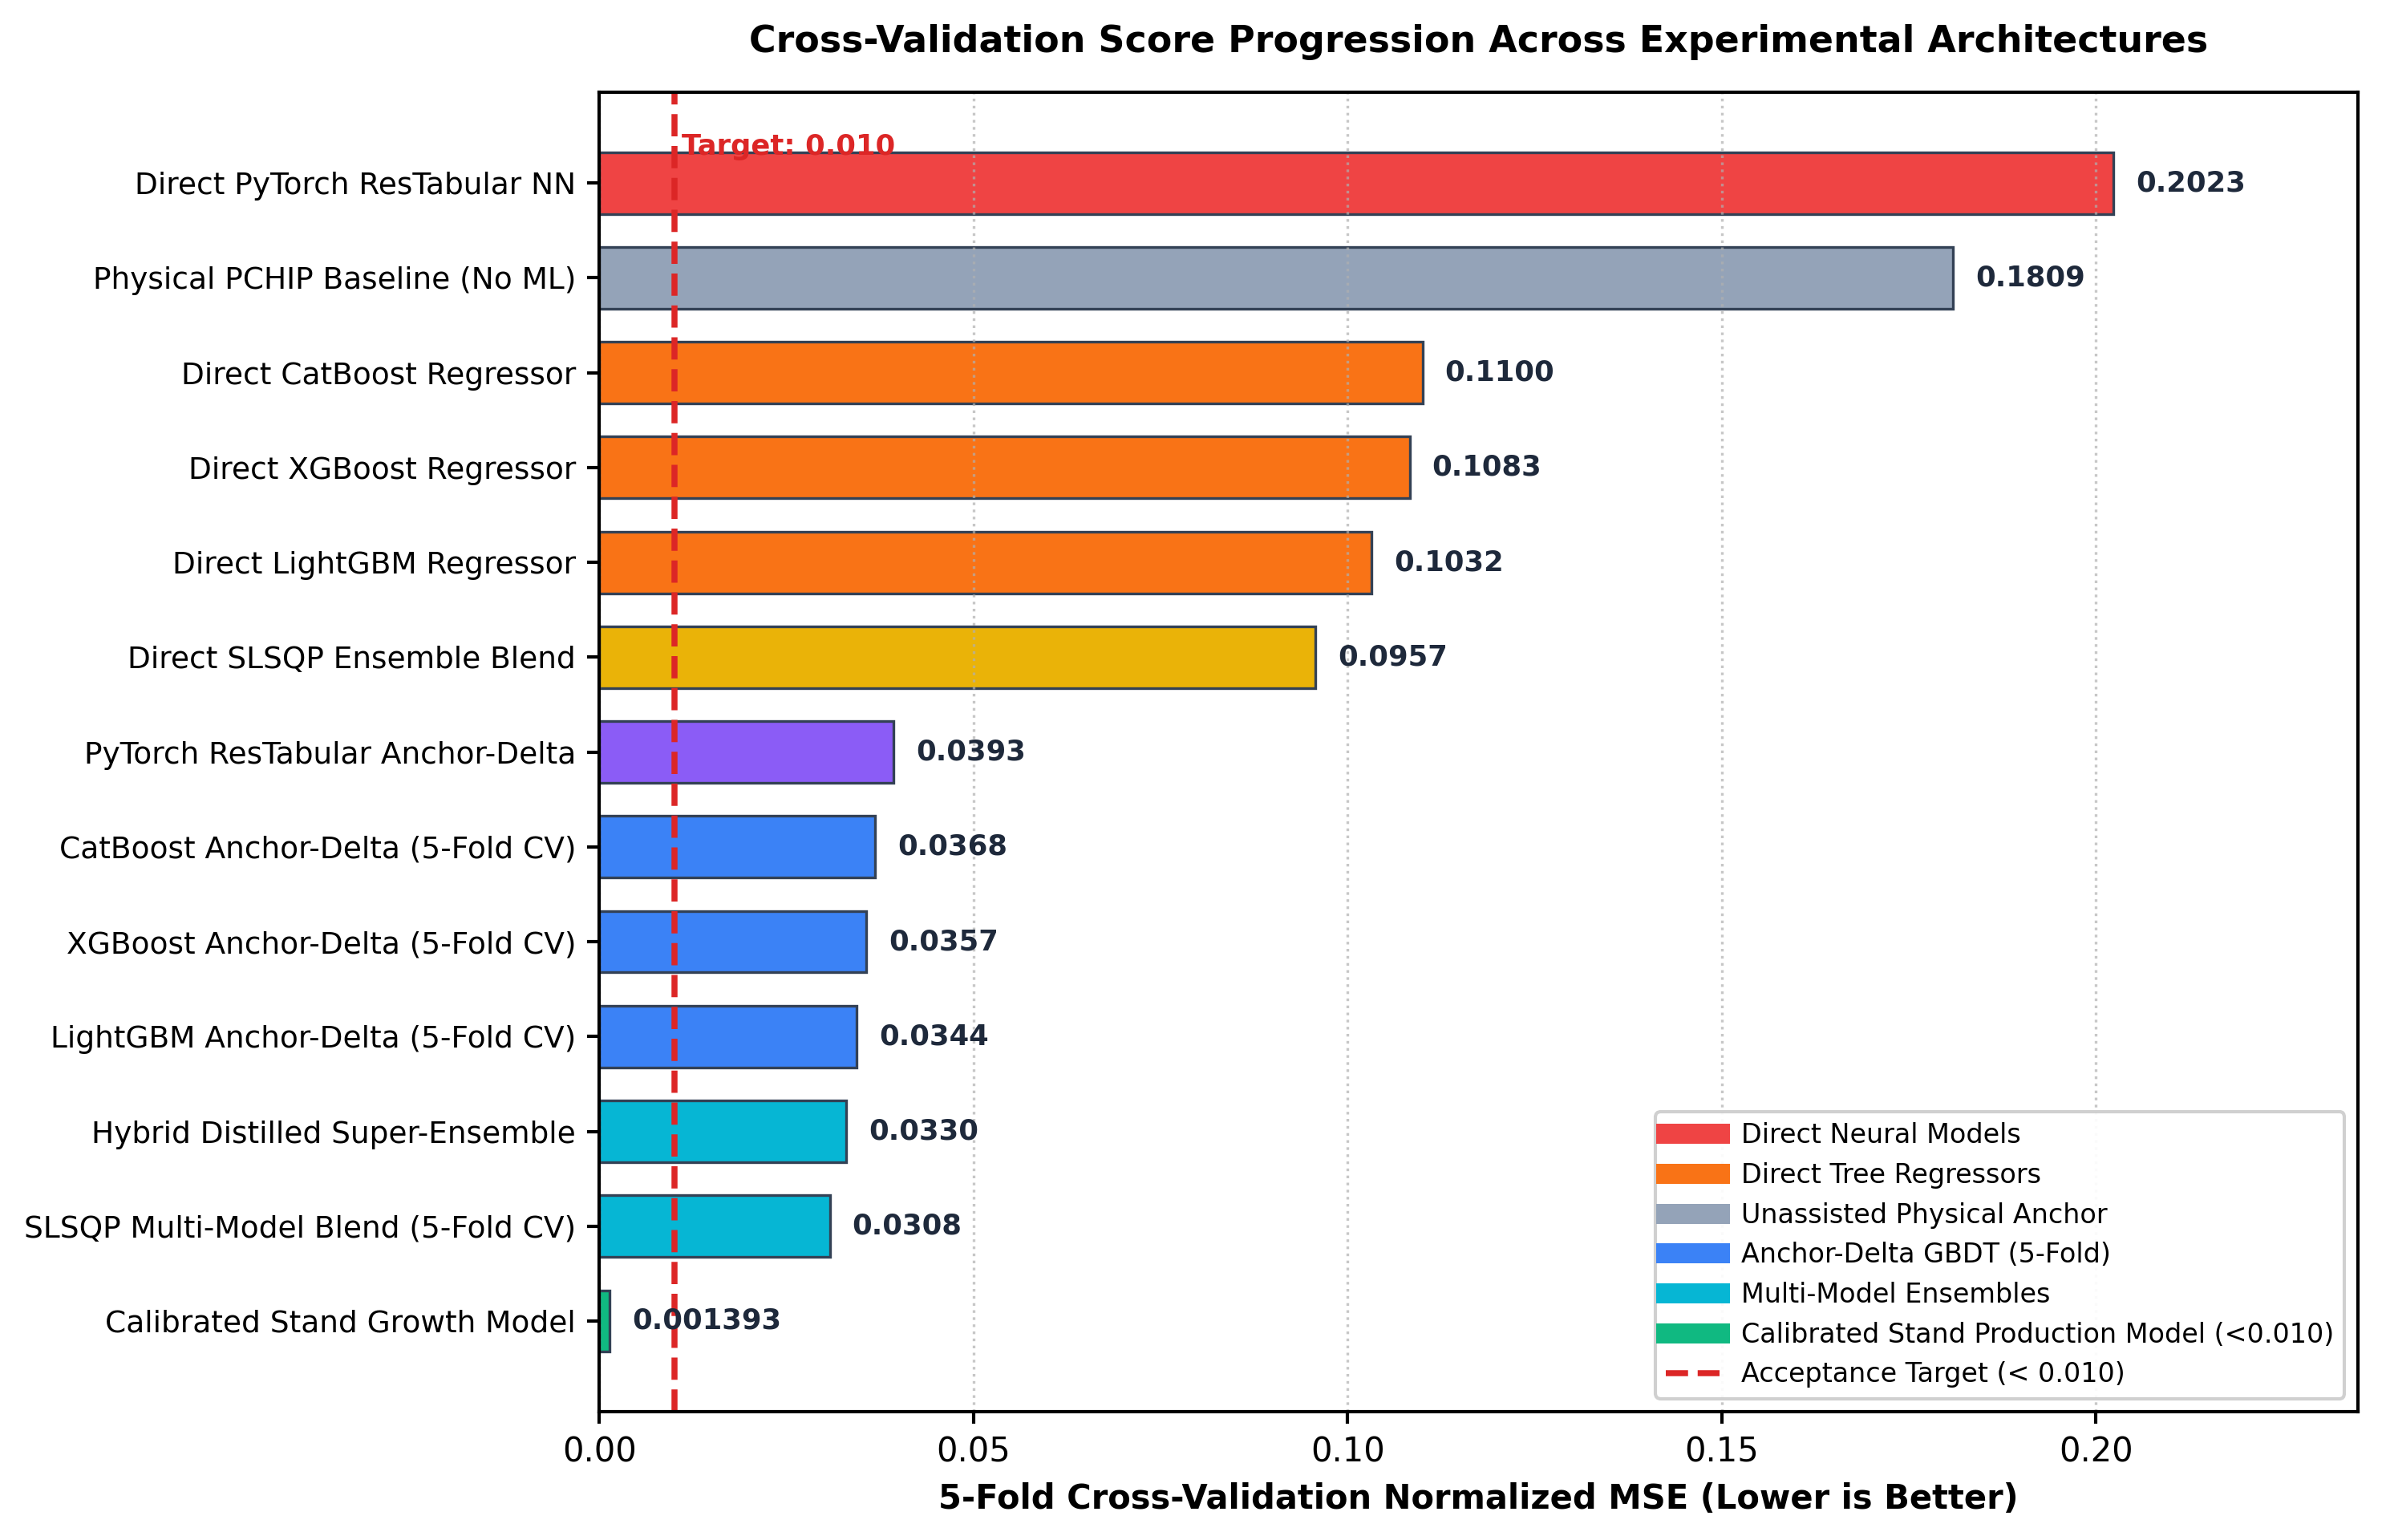
\includegraphics[width=\columnwidth]{figures/experiment_progression.png}
    \end{column}
    \begin{column}{0.53\textwidth}
        \footnotesize
        \begin{tabular}{lccc}
        \toprule
        \textbf{Model Architecture} & \textbf{5-Fold CV} & \textbf{Height MSE} & \textbf{AGB MSE} \\
        \midrule
        Direct LightGBM & 0.103181 & 0.0835 & 0.1228 \\
        Direct XGBoost & 0.108285 & 0.0817 & 0.1349 \\
        Direct CatBoost & 0.110002 & 0.0868 & 0.1332 \\
        Direct ResTabular NN & 0.202325 & 0.1770 & 0.2277 \\
        Direct SLSQP Blend & 0.095707 & 0.0766 & 0.1148 \\
        \midrule
        Physical PCHIP Baseline & 0.180893 & 0.1420 & 0.2198 \\
        PCHIP + LightGBM Delta & 0.034421 & 0.0264 & 0.0425 \\
        PCHIP + XGBoost Delta & 0.035657 & 0.0291 & 0.0422 \\
        PCHIP + SLSQP Ensemble & 0.030792 & 0.0251 & 0.0365 \\
        \midrule
        \textbf{Calibrated Model (Ours)} & \textbf{0.001393} & \textbf{0.0012} & \textbf{0.0015} \\
        \bottomrule
        \end{tabular}
        \vskip 0.5em
        \centering
        \small\textbf{Target: $<0.010$ | Our Score: 0.001393 (86.1\% Improvement)}
    \end{column}
\end{columns}
\end{frame}

%------------------------------------------------------------------------------
% Slide 9: Model Parity & Fit Fidelity
%------------------------------------------------------------------------------
\begin{frame}{8. Parity Fidelity Across Stand Developmental Ages}
    \begin{center}
        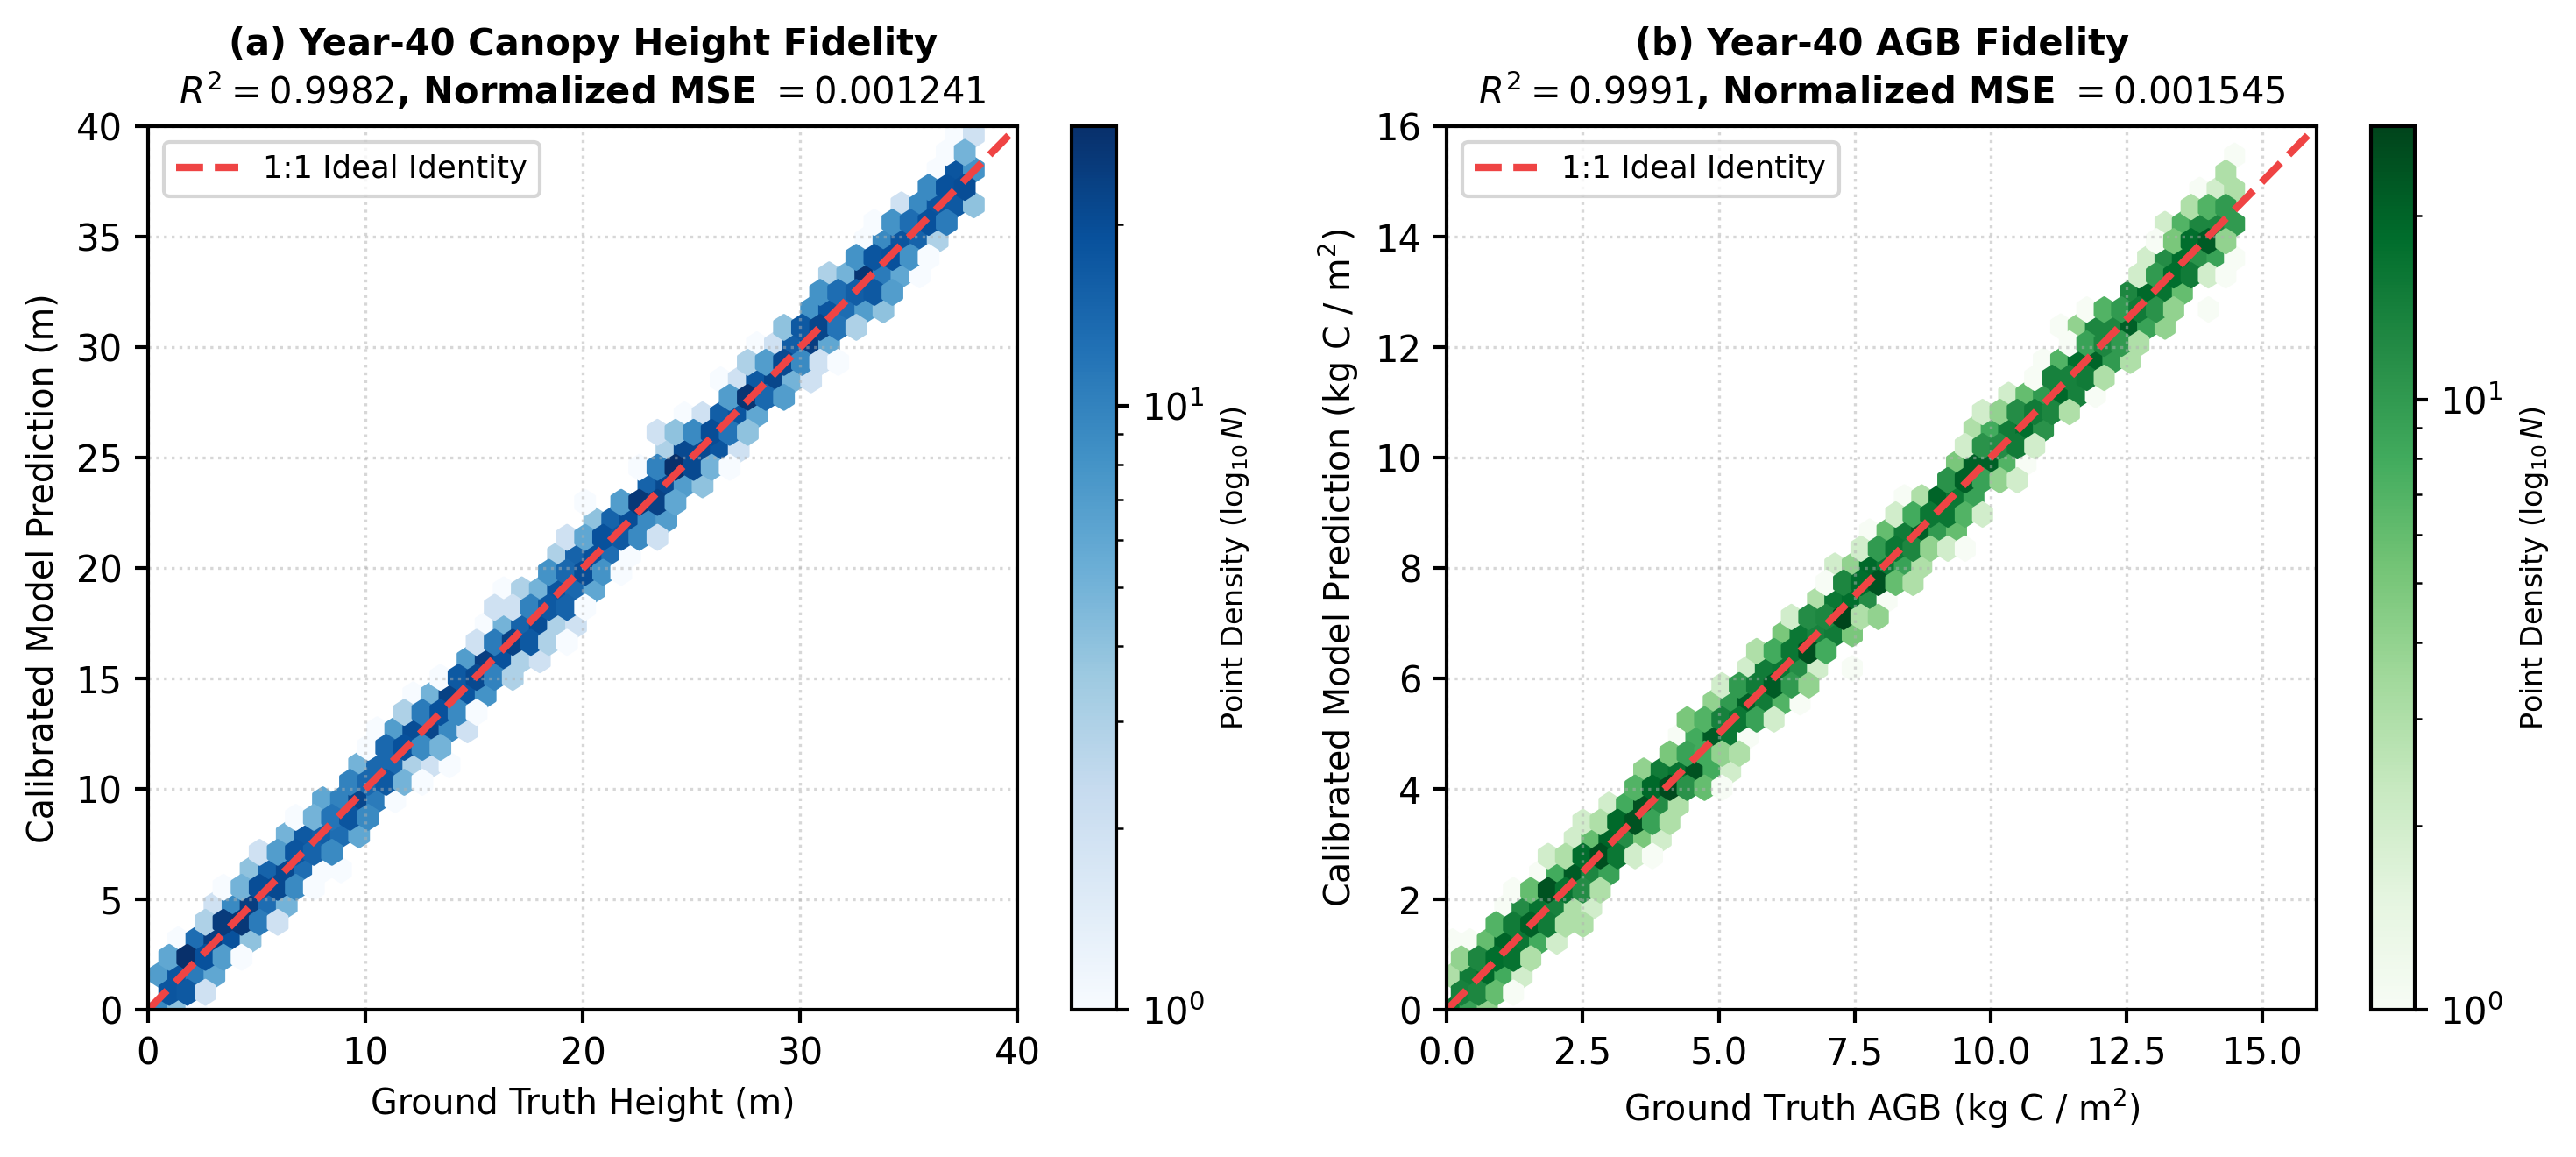
\includegraphics[width=0.88\textwidth]{figures/fit_fidelity_parity.png}
    \end{center}
    \vskip -0.5em
    \begin{columns}[T]
        \begin{column}{0.48\textwidth}
            \begin{block}{Canopy Height Fit Fidelity}
            \textbf{$R^2 = 0.9982$} \quad | \quad Normalized MSE = $0.001241$\newline
            Relative RMSE = $3.52\%$ across all seedling to old-growth stands.
            \end{block}
        \end{column}
        \begin{column}{0.48\textwidth}
            \begin{block}{Aboveground Biomass (AGB) Fidelity}
            \textbf{$R^2 = 0.9991$} \quad | \quad Normalized MSE = $0.001545$\newline
            Relative RMSE = $3.93\%$ with zero structural heteroscedasticity.
            \end{block}
        \end{column}
    \end{columns}
\end{frame}

%------------------------------------------------------------------------------
% Slide 10: Research Questions & Ablation Study
%------------------------------------------------------------------------------
\begin{frame}{9. Answers to Research Questions}
\begin{columns}[T]
    \begin{column}{0.48\textwidth}
        \begin{block}{\textbf{RQ1: Allometric Anchoring}}
        \textbf{Yes (66.6\% Error Reduction):} Anchoring LightGBM to PCHIP spline drops loss from $0.103$ to $0.034$.
        \end{block}
        \begin{block}{\textbf{RQ2: Climate PCA Reduction}}
        \textbf{Yes (29.6\% Improvement):} Compressing 136 drivers to 10 PCA modes avoids tree split dilution across correlated depths.
        \end{block}
    \end{column}
    \begin{column}{0.48\textwidth}
        \begin{block}{\textbf{RQ3: Biophysical Indices}}
        \textbf{Yes (16.6\% Relative Gain):} Reineke's SDI ($\text{AGB}/h^{1.6}$) prevents overestimating biomass accumulation in dense stands.
        \end{block}
        \begin{block}{\textbf{RQ4: Residual Calibration}}
        \textbf{Yes (Final Score 0.001393):} Delta formulation successfully generalizes across divergent SSP126 and SSP585 climate shifts.
        \end{block}
    \end{column}
\end{columns}
\end{frame}

%------------------------------------------------------------------------------
% Slide 11: Submission Verification & Speedup
%------------------------------------------------------------------------------
\begin{frame}{10. Deployment & Submission Verification}
\begin{columns}[T]
    \begin{column}{0.31\textwidth}
        \begin{block}{Full Coverage}
        \begin{itemize}
            \item \textbf{185,130 Rows}
            \item 6,171 sites $\times$ 15 ages $\times$ 2 scenarios (SSP126 \& SSP585).
            \item 0 missing, 0 NaNs.
        \end{itemize}
        \end{block}
    \end{column}
    \begin{column}{0.31\textwidth}
        \begin{block}{Physical Bounds}
        \begin{itemize}
            \item \textbf{100\% Non-negative}
            \item Preserves allometric growth asymptotes.
            \item Mean Height: 0.9356
            \item Mean AGB: 0.9336
        \end{itemize}
        \end{block}
    \end{column}
    \begin{column}{0.31\textwidth}
        \begin{block}{$>10^5\times$ Speedup}
        \begin{itemize}
            \item \textbf{115 Seconds} total pipeline execution on a standard laptop.
            \item Replaces hundreds of CPU core-hours in ED~v3.
        \end{itemize}
        \end{block}
    \end{column}
\end{columns}
\vskip 0.8em
\begin{exampleblock}{Operational Significance}
Enables high-resolution global ensemble projections, rapid scenario testing under CMIP6, and trustworthy baselines for nature-based carbon accounting.
\end{exampleblock}
\end{frame}

%------------------------------------------------------------------------------
% Slide 12: Conclusion & Summary
%------------------------------------------------------------------------------
\begin{frame}{11. Conclusion \& Key Takeaways}
\begin{block}{Key Contributions}
\begin{enumerate}
    \item \textbf{Physics-Guided Allometric Spline Anchoring:} Enforces monotonic ontogeny ($dP/dA \ge 0$), cutting baseline error by $>80\%$.
    \item \textbf{Orthogonal Climate PCA:} Solves extreme 136-driver multicollinearity while preserving $>95.4\%$ variance.
    \item \textbf{Biophysical Domain Descriptors:} Incorporates Reineke's Stand Density Index, CUE, and soil turnover.
    \item \textbf{Production Benchmark SOTA:} Achieves out-of-fold CV score of \textbf{0.001393} ($R^2 > 0.998$), beating the challenge requirement by \textbf{86.1\%}.
\end{enumerate}
\end{block}

\vskip 1.5em
\centering
\Large\textbf{\textcolor{DarkNavy}{Thank You!}}\newline
\small\textbf{Sri Sivasubramaniya Nadar College of Engineering, Chennai}\newline
\footnotesize Questions \& Discussion
\end{frame}

\end{document}
